% GNUPLOT: LaTeX picture with Postscript
\begingroup
  \makeatletter
  \providecommand\color[2][]{%
    \GenericError{(gnuplot) \space\space\space\@spaces}{%
      Package color not loaded in conjunction with
      terminal option `colourtext'%
    }{See the gnuplot documentation for explanation.%
    }{Either use 'blacktext' in gnuplot or load the package
      color.sty in LaTeX.}%
    \renewcommand\color[2][]{}%
  }%
  \providecommand\includegraphics[2][]{%
    \GenericError{(gnuplot) \space\space\space\@spaces}{%
      Package graphicx or graphics not loaded%
    }{See the gnuplot documentation for explanation.%
    }{The gnuplot epslatex terminal needs graphicx.sty or graphics.sty.}%
    \renewcommand\includegraphics[2][]{}%
  }%
  \providecommand\rotatebox[2]{#2}%
  \@ifundefined{ifGPcolor}{%
    \newif\ifGPcolor
    \GPcolorfalse
  }{}%
  \@ifundefined{ifGPblacktext}{%
    \newif\ifGPblacktext
    \GPblacktexttrue
  }{}%
  % define a \g@addto@macro without @ in the name:
  \let\gplgaddtomacro\g@addto@macro
  % define empty templates for all commands taking text:
  \gdef\gplbacktext{}%
  \gdef\gplfronttext{}%
  \makeatother
  \ifGPblacktext
    % no textcolor at all
    \def\colorrgb#1{}%
    \def\colorgray#1{}%
  \else
    % gray or color?
    \ifGPcolor
      \def\colorrgb#1{\color[rgb]{#1}}%
      \def\colorgray#1{\color[gray]{#1}}%
      \expandafter\def\csname LTw\endcsname{\color{white}}%
      \expandafter\def\csname LTb\endcsname{\color{black}}%
      \expandafter\def\csname LTa\endcsname{\color{black}}%
      \expandafter\def\csname LT0\endcsname{\color[rgb]{1,0,0}}%
      \expandafter\def\csname LT1\endcsname{\color[rgb]{0,1,0}}%
      \expandafter\def\csname LT2\endcsname{\color[rgb]{0,0,1}}%
      \expandafter\def\csname LT3\endcsname{\color[rgb]{1,0,1}}%
      \expandafter\def\csname LT4\endcsname{\color[rgb]{0,1,1}}%
      \expandafter\def\csname LT5\endcsname{\color[rgb]{1,1,0}}%
      \expandafter\def\csname LT6\endcsname{\color[rgb]{0,0,0}}%
      \expandafter\def\csname LT7\endcsname{\color[rgb]{1,0.3,0}}%
      \expandafter\def\csname LT8\endcsname{\color[rgb]{0.5,0.5,0.5}}%
    \else
      % gray
      \def\colorrgb#1{\color{black}}%
      \def\colorgray#1{\color[gray]{#1}}%
      \expandafter\def\csname LTw\endcsname{\color{white}}%
      \expandafter\def\csname LTb\endcsname{\color{black}}%
      \expandafter\def\csname LTa\endcsname{\color{black}}%
      \expandafter\def\csname LT0\endcsname{\color{black}}%
      \expandafter\def\csname LT1\endcsname{\color{black}}%
      \expandafter\def\csname LT2\endcsname{\color{black}}%
      \expandafter\def\csname LT3\endcsname{\color{black}}%
      \expandafter\def\csname LT4\endcsname{\color{black}}%
      \expandafter\def\csname LT5\endcsname{\color{black}}%
      \expandafter\def\csname LT6\endcsname{\color{black}}%
      \expandafter\def\csname LT7\endcsname{\color{black}}%
      \expandafter\def\csname LT8\endcsname{\color{black}}%
    \fi
  \fi
  \setlength{\unitlength}{0.0500bp}%
  \begin{picture}(6480.00,4320.00)%
    \gplgaddtomacro\gplbacktext{%
      \csname LTb\endcsname%
      \put(1519,704){\makebox(0,0)[r]{\strut{}-0.3}}%
      \put(1519,1374){\makebox(0,0)[r]{\strut{}-0.2}}%
      \put(1519,2045){\makebox(0,0)[r]{\strut{}-0.1}}%
      \put(1519,2715){\makebox(0,0)[r]{\strut{} 0}}%
      \put(1519,3386){\makebox(0,0)[r]{\strut{} 0.1}}%
      \put(1519,4056){\makebox(0,0)[r]{\strut{} 0.2}}%
      \put(2070,484){\makebox(0,0){\strut{}-40}}%
      \put(2908,484){\makebox(0,0){\strut{}-20}}%
      \put(3746,484){\makebox(0,0){\strut{} 0}}%
      \put(4584,484){\makebox(0,0){\strut{} 20}}%
      \put(5422,484){\makebox(0,0){\strut{} 40}}%
      \put(881,2380){\rotatebox{90}{\makebox(0,0){\strut{}\sf Lock error signal (V)}}}%
      \put(3746,154){\makebox(0,0){\strut{}\sf Detuning (MHz)}}%
      \put(4079,3520){\makebox(0,0)[l]{\strut{}\sf \small 5.6$\pm$0.1 MHz}}%
      \put(2070,3184){\makebox(0,0)[l]{\strut{}\sf \small pk-pk: 1.3 MHz}}%
      \put(2070,2983){\makebox(0,0)[l]{\strut{}\sf \small rms  :  210 kHz}}%
      \put(2070,3453){\makebox(0,0)[l]{\strut{}\sf \small Locked linewidth:}}%
    }%
    \gplgaddtomacro\gplfronttext{%
    }%
    \gplgaddtomacro\gplbacktext{%
      \csname LTb\endcsname%
      \put(4289,1148){\makebox(0,0)[r]{\strut{}\tiny -100}}%
      \put(4289,1408){\makebox(0,0)[r]{\strut{}\tiny -50}}%
      \put(4289,1668){\makebox(0,0)[r]{\strut{}\tiny 0}}%
      \put(4289,1927){\makebox(0,0)[r]{\strut{}\tiny 50}}%
      \put(4289,2187){\makebox(0,0)[r]{\strut{}\tiny 100}}%
      \put(4463,1038){\makebox(0,0){\strut{}\tiny -0.5}}%
      \put(5004,1038){\makebox(0,0){\strut{}\tiny 0}}%
      \put(5546,1038){\makebox(0,0){\strut{}\tiny 0.5}}%
      \put(4047,1667){\rotatebox{90}{\makebox(0,0){\strut{}\sf \tiny mV}}}%
      \put(5004,927){\makebox(0,0){\strut{}\sf \tiny MHz}}%
      \put(5004,2418){\makebox(0,0){\strut{}\sf \tiny Error signal zero crossing}}%
      \put(4571,2291){\makebox(0,0)[l]{\strut{}\sf \tiny 127.64 mV/MHz}}%
    }%
    \gplgaddtomacro\gplfronttext{%
    }%
    \gplgaddtomacro\gplbacktext{%
      \csname LTb\endcsname%
      \put(2086,1129){\makebox(0,0)[r]{\strut{}\tiny -100}}%
      \put(2086,1396){\makebox(0,0)[r]{\strut{}\tiny -50}}%
      \put(2086,1662){\makebox(0,0)[r]{\strut{}\tiny 0}}%
      \put(2086,1929){\makebox(0,0)[r]{\strut{}\tiny 50}}%
      \put(2086,2195){\makebox(0,0)[r]{\strut{}\tiny 100}}%
      \put(2818,2305){\makebox(0,0){\strut{}\sf \tiny Error (mV), $\Delta$ t=1 s}}%
    }%
    \gplgaddtomacro\gplfronttext{%
    }%
    \gplbacktext
    \put(0,0){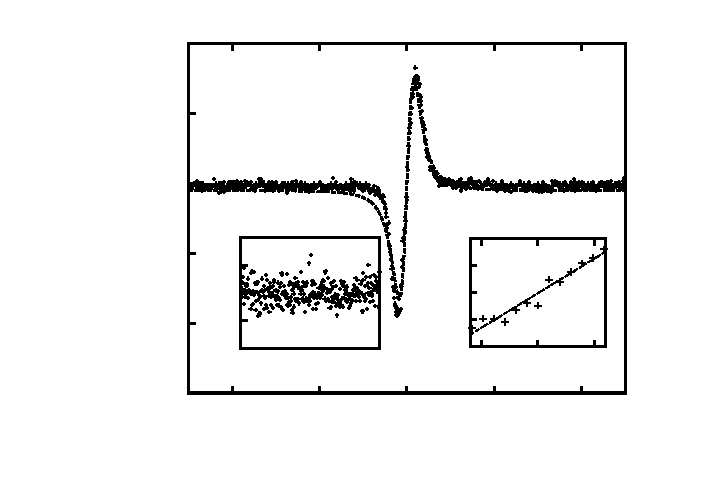
\includegraphics{lockfig}}%
    \gplfronttext
  \end{picture}%
\endgroup
